\documentclass[a4paper,11pt]{article}

\usepackage[utf8]{inputenc}
\usepackage[T1]{fontenc} % LY1 also works
\usepackage[margin=1in]{geometry}

%% Font settings suggested by fbb documentation.
\usepackage{textcomp} % to get the right copyright, etc.
\usepackage[lining,tabular]{fbb} % so math uses tabular lining figures
\usepackage[scaled=.95,type1]{cabin} % sans serif in style of Gill Sans
\usepackage[varqu,varl]{zi4}% inconsolata typewriter
\useosf % change normal text to use proportional oldstyle figures
%\usetosf would provide tabular oldstyle figures in text

\usepackage{microtype}
\usepackage{siunitx}
\DeclareSIUnit{\belmilliwatt}{Bm}
\DeclareSIUnit{\dBm}{\deci\belmilliwatt}
\sisetup{range-phrase=--, range-units=single, binary-units = true}
\usepackage{graphicx}
\usepackage{tikz}
%\usepackage{hyperref}
\usetikzlibrary{arrows, shadows}
\tikzset{%
  cascaded/.style = {%
    general shadow = {%
      shadow scale = 1,
      shadow xshift = -1ex,
      shadow yshift = 1ex,
      draw,
      thick,
      fill = white},
    general shadow = {%
      shadow scale = 1,
      shadow xshift = -.5ex,
      shadow yshift = .5ex,
      draw,
      thick,
      fill = white},
    fill = white, 
    draw,
    thick,
    minimum width = 1.5cm,
    minimum height = 2cm}}
    
\usepackage{enumitem}
\setlist{leftmargin=*}
\usepackage{listings}
\lstset{
	basicstyle=\ttfamily,
	frame=single,
	breaklines=true,
	morecomment=[l][\color{green}]{\#},
}
\usepackage[os=win]{menukeys}
\renewmenumacro{\keys}[+]{shadowedroundedkeys}

\usepackage{booktabs,caption}
\usepackage[flushleft]{threeparttable}
\newcolumntype{L}[1]{>{\raggedright\let\newline\\\arraybackslash\hspace{0pt}}m{#1}}
\newcolumntype{C}[1]{>{\centering\let\newline\\\arraybackslash\hspace{0pt}}m{#1}}
\newcolumntype{R}[1]{>{\raggedleft\let\newline\\\arraybackslash\hspace{0pt}}m{#1}}
\usepackage{tabularx} 

\usepackage{stackengine}
\usepackage{scalerel}
\usepackage{xcolor,mdframed}

\newcommand\danger[1][5ex]{%
  \renewcommand\stacktype{L}%
  \scaleto{\stackon[1.3pt]{\color{red}$\triangle$}{\tiny !}}{#1}%
}

\newenvironment{important}[1][]{%
   \begin{mdframed}[%
      backgroundcolor={red!15}, hidealllines=true,
      skipabove=0.7\baselineskip, skipbelow=0.7\baselineskip,
      splitbottomskip=2pt, splittopskip=4pt, #1]%
   \makebox[0pt]{% ignore the withd of !
      \smash{% ignor the height of !
         %\fontsize{32pt}{32pt}\selectfont% make the ! bigger
         \hspace*{-45pt}% move ! to the left
         \raisebox{-5pt}{% move ! up a little
            {\danger}% type the bold red !
         }%
      }%
   }%
}{\end{mdframed}}

\newcommand\info[1][5ex]{%
  \renewcommand\stacktype{L}%
  \scaleto{\stackon[1.2pt]{\color{blue}$\bigcirc$}{\raisebox{-1.5pt}{\small i}}}{#1}%
}

\newenvironment{information}[1][]{%
   \begin{mdframed}[%
      backgroundcolor={blue!15}, hidealllines=true,
      skipabove=0.7\baselineskip, skipbelow=0.7\baselineskip,
      splitbottomskip=2pt, splittopskip=4pt, #1]%
   \makebox[0pt]{% ignore the withd of !
      \smash{% ignor the height of !
         %\fontsize{32pt}{32pt}\selectfont% make the ! bigger
         \hspace*{-45pt}% move ! to the left
         \raisebox{-5pt}{% move ! up a little
            {\info}% type the bold red !
         }%
      }%
   }%
}{\end{mdframed}}

\usepackage{hyperref}
\newcommand{\vna}{VNA}

\title{\vna{} User Manual}
%\author{Jan Käberich (\url{j.kaeberich@gmx.de})}
\begin{document}
\maketitle

%\begin{abstract}
%The Testcard is a platform for the characterization of small energy sources. It is able to charge/discharge up to eight energy sources with a predefined pattern and record their voltages.
%\end{abstract}

\setcounter{tocdepth}{2}
\tableofcontents
\clearpage

%\section*{Nomenclature}
%
%\begin{description}
%\item[Testcard] Board with the hardware to characterize up to eight energy sources.
%\item[CLI] Command Line Interface. Program running on the computer which controls the testcard.
%\item[Channel] One of the eight measurement units on the testcard.
%\begin{description}
%\item[Voltage] Voltage of the energy source connected to the channel.
%\item[Current] Current flowing through the energy source connected to the channel. Defined as the current flowing from the energy source to the testcard, thus the source is discharged for positive and charged for negative values.
%\end{description}
%\item[Load] Application of a current at the channels for a specified timespan.
%\item[Measurement] Single measurement of channel voltages at a specified point in time.
%\item[Trace] Periodic measurement of channel voltages.
%\item[Sequence] A combination of loads, measurements and traces.
%\end{description}

\section{Overview}

\begin{tikzpicture}
\begin{scope}[xshift=1.5cm]
    \node[anchor=south west,inner sep=0] (image) at (0,0) {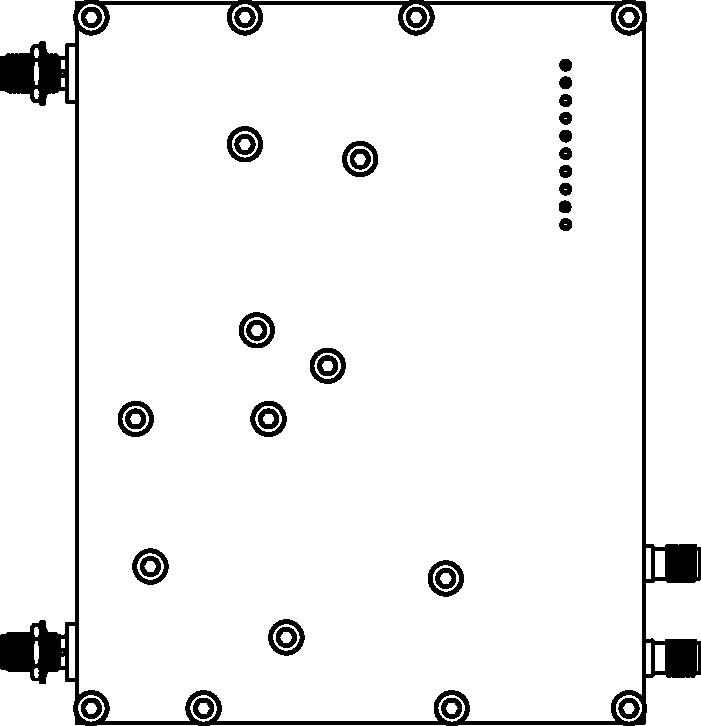
\includegraphics[width=0.76\textwidth]{TopDrawing.pdf}};
    \begin{scope}[x={(image.south east)},y={(image.north west)}]
		\node [anchor=south, align=center] (port1) at (0,1) {Port 1};
		\node [anchor=south, align=center] (port2) at (0,0.2) {Port 2};
		\node [anchor=west, align=center] (leds) at (1.05,0.8) {LEDs\\ \footnotesize Ready\\ \footnotesize Debug\\ \footnotesize Port1\\ \footnotesize Port2\\ \footnotesize Ext. Reference\\ \footnotesize Source unlocked\\ \footnotesize LO unlocked\\ \footnotesize FPGA unlocked\\ \footnotesize Booting\\ \footnotesize Power};
		\node [anchor=west, align=center] (usb) at (1.1,0.4) {USB};
		\node [anchor=west, align=center] (refout) at (1.1,0.2) {Reference\\Output};
		\node [anchor=west, align=center] (refin) at (1.1,0) {Reference \\Input};

        \draw [-*, ultra thick, gray] (port1) to[] (0.02,0.89);
        \draw [-*, ultra thick, gray] (port2) to[] (0.02,0.09);
        \draw [-*, ultra thick, gray] (leds) to[] (0.8,0.84);
        \draw [-*, ultra thick, gray] (usb) to[] (0.91,0.5);
        \draw [-*, ultra thick, gray] (refout) to[] (0.97,0.23);
        \draw [-*, ultra thick, gray] (refin) to[] (0.97,0.1);
    \end{scope}
\end{scope}
\end{tikzpicture}%

\subsection{USB}
The \vna{} uses a USB-C connector as the power supply and for data transmission. The hardware supports the USB power delivery standard\footnote{Work in progress, the device will not negotiate USB-PD yet}, requires \SI{5}{\volt} and draws up to \SI{1.2}{\ampere} of current.

The implemented USB device is limited to USB 2.0 Fullspeed and data transmission will work with any USB 2.0 or 3.0 port (no USB-C required). However, the current consumption exceeds the specifications for USB 2.0 and 3.0 ports and the \vna{} may be unable to fully boot when the USB host limits the current.
\subsection{RF ports}
RF connector to connect the DUT. Both ports are identical and the device architecture support full S-Parameter measurements (S11, S21, S12 and S22).
\begin{important}
The RF ports have no input protection, do not apply a signal with more than +\SI{10}{\dBm} of power.
\end{important}
\subsection{LEDs}
Ten LEDs indicate the status:
\begin{description}
\item [Ready (green)] Indicates fully booted \vna{}, ready to take measurements
\item [Debug (green)] Not used at the moment
\item [Port 1 (green)] Active output signal on port 1
\item [Port 2 (green)] Active output signal on port 2
\item [Ext. Reference (green)] External reference in use
\item [Source unlocked (red)] The source PLL failed to lock (it may turn on briefly during a sweep, this is not a problem)
\item [LO unlocked (red)] The 1.LO PLL failed to lock (it may turn on briefly during a sweep, this is not a problem)
\item [FPGA unlocked (red)] The FPGA clock PLL failed to lock
\item [Booting (red)] Indicates boot process, also used for error codes
\item [Power (green)] USB power valid
\end{description}
\subsection{Reference Output}
Optional reference output port (user selectable \SI{10}{\mega\hertz} or \SI{100}{\mega\hertz}). The output power is approximately +\SI{3}{\dBm}.
\subsection{Reference Input}
High impedance reference input port. When applying a \SI{10}{\mega\hertz} input signal, it can be used to overwrite the internal TCXO.
\begin{information}
Due to the high impedance input, the external input may detect a valid signal when picking up external radiation. If this is a problem, either terminate the reference input connector or disable automatic reference switching.
\end{information}

\section{Getting started}
\begin{enumerate}
\item Connect the \vna{} to a computer using the USB port. After a couple of seconds, only the "Power" and "Ready" LEDs should stay on. If the "Ready" LED does not turn on or the "Booting" LED indicates an error code, there is a problem und the device will not function properly. See section~\ref{troubleshooting} for possible solutions.
\item Start the PC application to connect to the \vna{}. The window should look similar to this:
\makebox[\textwidth][c]{
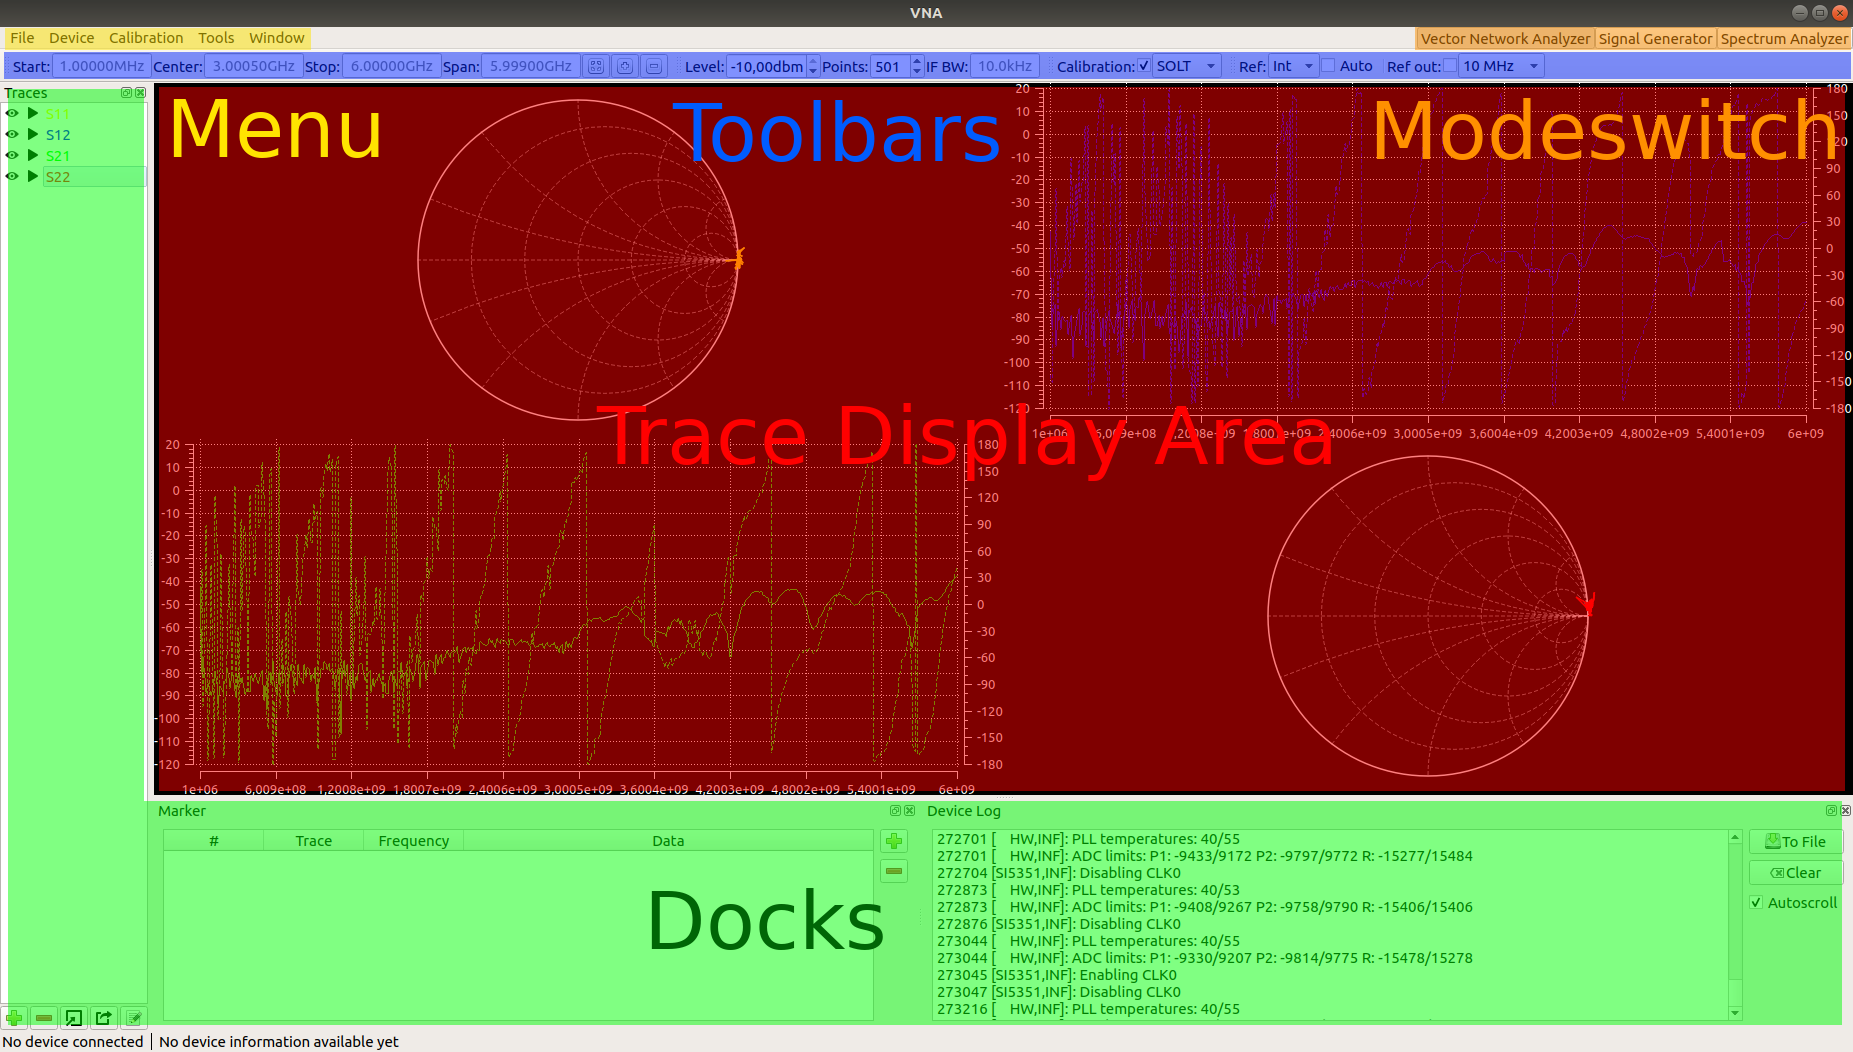
\includegraphics[width=\textwidth]{ApplicationOverview.png}
}
\end{enumerate}
\subsection{GUI elements types}
The \vna{} application is made up of six areas containing different types of control:
\begin{itemize}
\item The \textbf{Trace Display Area} shows the measured data in various diagrams.
\item The \textbf{Toolbars} provide access to commonly used device settings.
\item The \textbf{Menu} at the top left handles less common settings or more complex actions (often with additional popup windows).
\item The \textbf{Docks} mostly provide access to display related settings such as traces and markers.
\item The \textbf{Statusbar} at the bottom show some basic informations about the connected device.
\item The \textbf{Modeswitch} at the top right allows changing the \vna{} operating mode. Although it is primarily designed as a vector network analyzer, the hardware architecture allow some other operating modes with certain limitations.
\end{itemize}
Depending on the current operating mode, the available toolbars, docks and menu entries change. It is also possible to rearrange the docks and toolbars.

\subsection{Common GUI elements}
Certain control elements are always available, regardless of the selected mode. They control settings of the \vna{} that are not specific to any of the operating modes.
\subsubsection{Reference Toolbar}
The reference toolbar controls the external reference output as well as the input.
\begin{center}

\includegraphics[height=0.7cm]{ToolbarReference.png}
\end{center}
The reference can be set to "Int" (internal TCXO), "Ext" (external \SI{10}{\mega\hertz} signal) or to automatic mode. In automatic mode, the reference will switch to the external input when a signal is detected, otherwise it will use the internal TCXO.

The external reference output may either be disabled or set to \SI{10}{\mega\hertz} or \SI{100}{\mega\hertz}.

\subsubsection{Device Log Dock}
This dock shows the debug output of the \vna{} (the same messages as on the internal UART port). It may help to identify problems, otherwise it is not required for operation.
\begin{center}
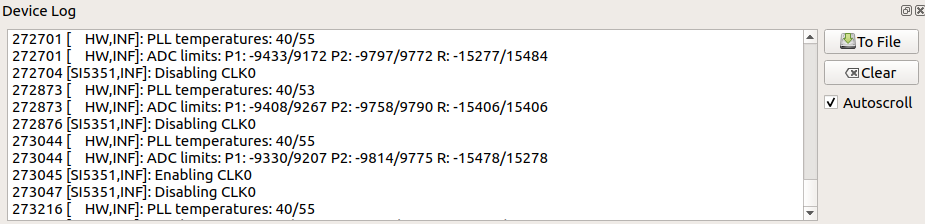
\includegraphics[width=\textwidth]{DockDeviceLog.png}
\end{center}

\subsubsection{Device Menu}
The device menu controls the connection state, allows low level hardware access and to perform firmware updates:
\begin{itemize}
\item \textbf{Update Device List:} Scans the USB port for connected devices. Clicking this action simply updates the list of devices, no connection is established.
\item \textbf{Connect to:} Select which \vna{} to connect to. Different devices are identified by their serial number.
\item \textbf{Disconnect:} Disconnect from the \vna{}.
\item \textbf{Manual Control:} Starts the manual control dialog in which all hardware settings are accessible (mostly used for testing purposes):
\begin{center}
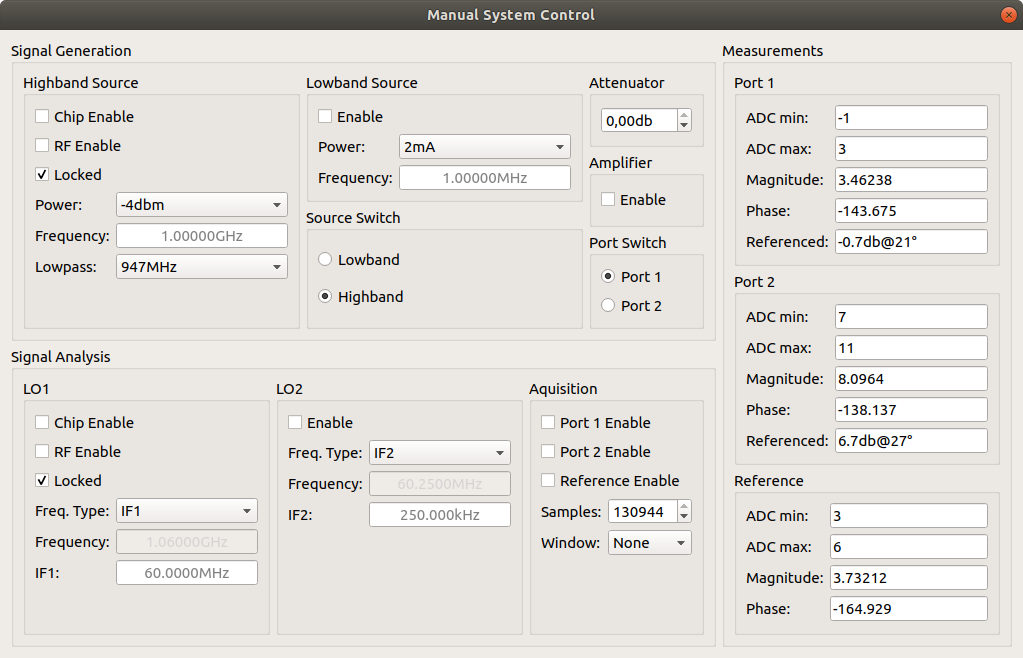
\includegraphics[width=\textwidth]{DialogManualControl.png}
\end{center}
\item \textbf{Firmware Update:} Load a new microcontroller firmware and FPGA configuration into the \vna{}. Do not disconnect power while updating the firmware!
\begin{center}
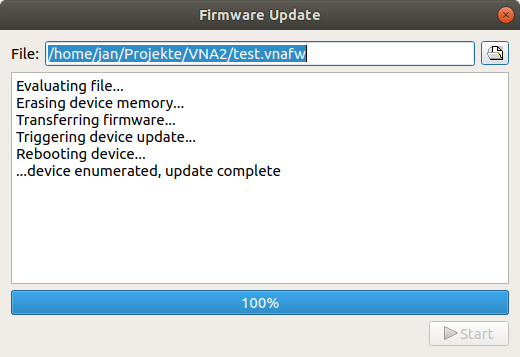
\includegraphics[width=0.6\textwidth]{DialogFirmwareUpdate.png}
\end{center}
\end{itemize}

\subsubsection{Window Menu}
The window menu allows hiding not needed toolbars and docks. It also contains some application preferences.

\section{Operating Modes}
\subsection{Vector Network Analyzer}
In this operating mode, the \vna{} takes S-parameter measurements. A source signal is generated and alternately applied to the RF ports. The incoming signal at both RF ports is measured, resulting in the four S-parameters S11 and S21 (when the source signal is routed to port 1) as well as S12 and S22 (when it is routed to port 2).
\subsection{Signal Generator}
\subsection{Spectrum Analyzer}

\section{Troubleshooting}
\label{troubleshooting}
If the was an error in the boot process, the "Booting" LED will blink an error code repeatedly:
\begin{center}
\begin{threeparttable}
\begin{tabularx}{\textwidth}{L{1cm}|X|L{7cm}}
    \toprule
    \textbf{Error Code} & \textbf{Meaning} & \textbf{Possible solution}\\
     \hline
      1   	&      Failed to detect FLASH memory  & \\
    \hline
      2   	&      Invalid FLASH content  & Perform firmware update\\
    \hline
      3   	&      Failed to configure FPGA & Check FPGA bitstream generator settings\\
    \hline
      4   	&      Hardware initialization failed & Verify that FPGA bitstream and uC firmware are created from the same release\\
      \bottomrule
\end{tabularx}
\end{threeparttable}
\end{center}
\end{document}
